%!TEX root = ../main.tex
%=========================================================

\section{Performance Evaluation}\label{sec:eval}

\subsection{Ticket table occupancy evaluation}

- Ticket table occupancy  and waiting time evaluation

\subsection{Network simulator evaluation}

\subsubsection{Evaluation Setup and Assumptions}


For the network performance evaluation we extended the existing 
a large-scale peer-to-peer network simulatior PeerSim~\cite{p2p09-peersim}.
We implemented the current Discv5 protocol by modyfing the existing PeerSim Kademlia implementation with the features of the Kademlia version used by the Ethereum network and our proposed mechanisms.

\subsubsection{Results}

\paragraph{\bf{Active registrations}:}

\begin{figure}[h!]
\centering
%\epsfig{file=imgs/eval/scen5.pdf, width=0.45\textwidth}
\includegraphics[width=0.3\textwidth]{img/eval/registration_origin.png}
\caption{Active Registrations}
\label{fig:regs}
\vspace{-0.15in}
\end{figure}

\paragraph{\bf{Network load}:}


\begin{figure}[!h]
\centering
\subfigure[{Number of messages}]{
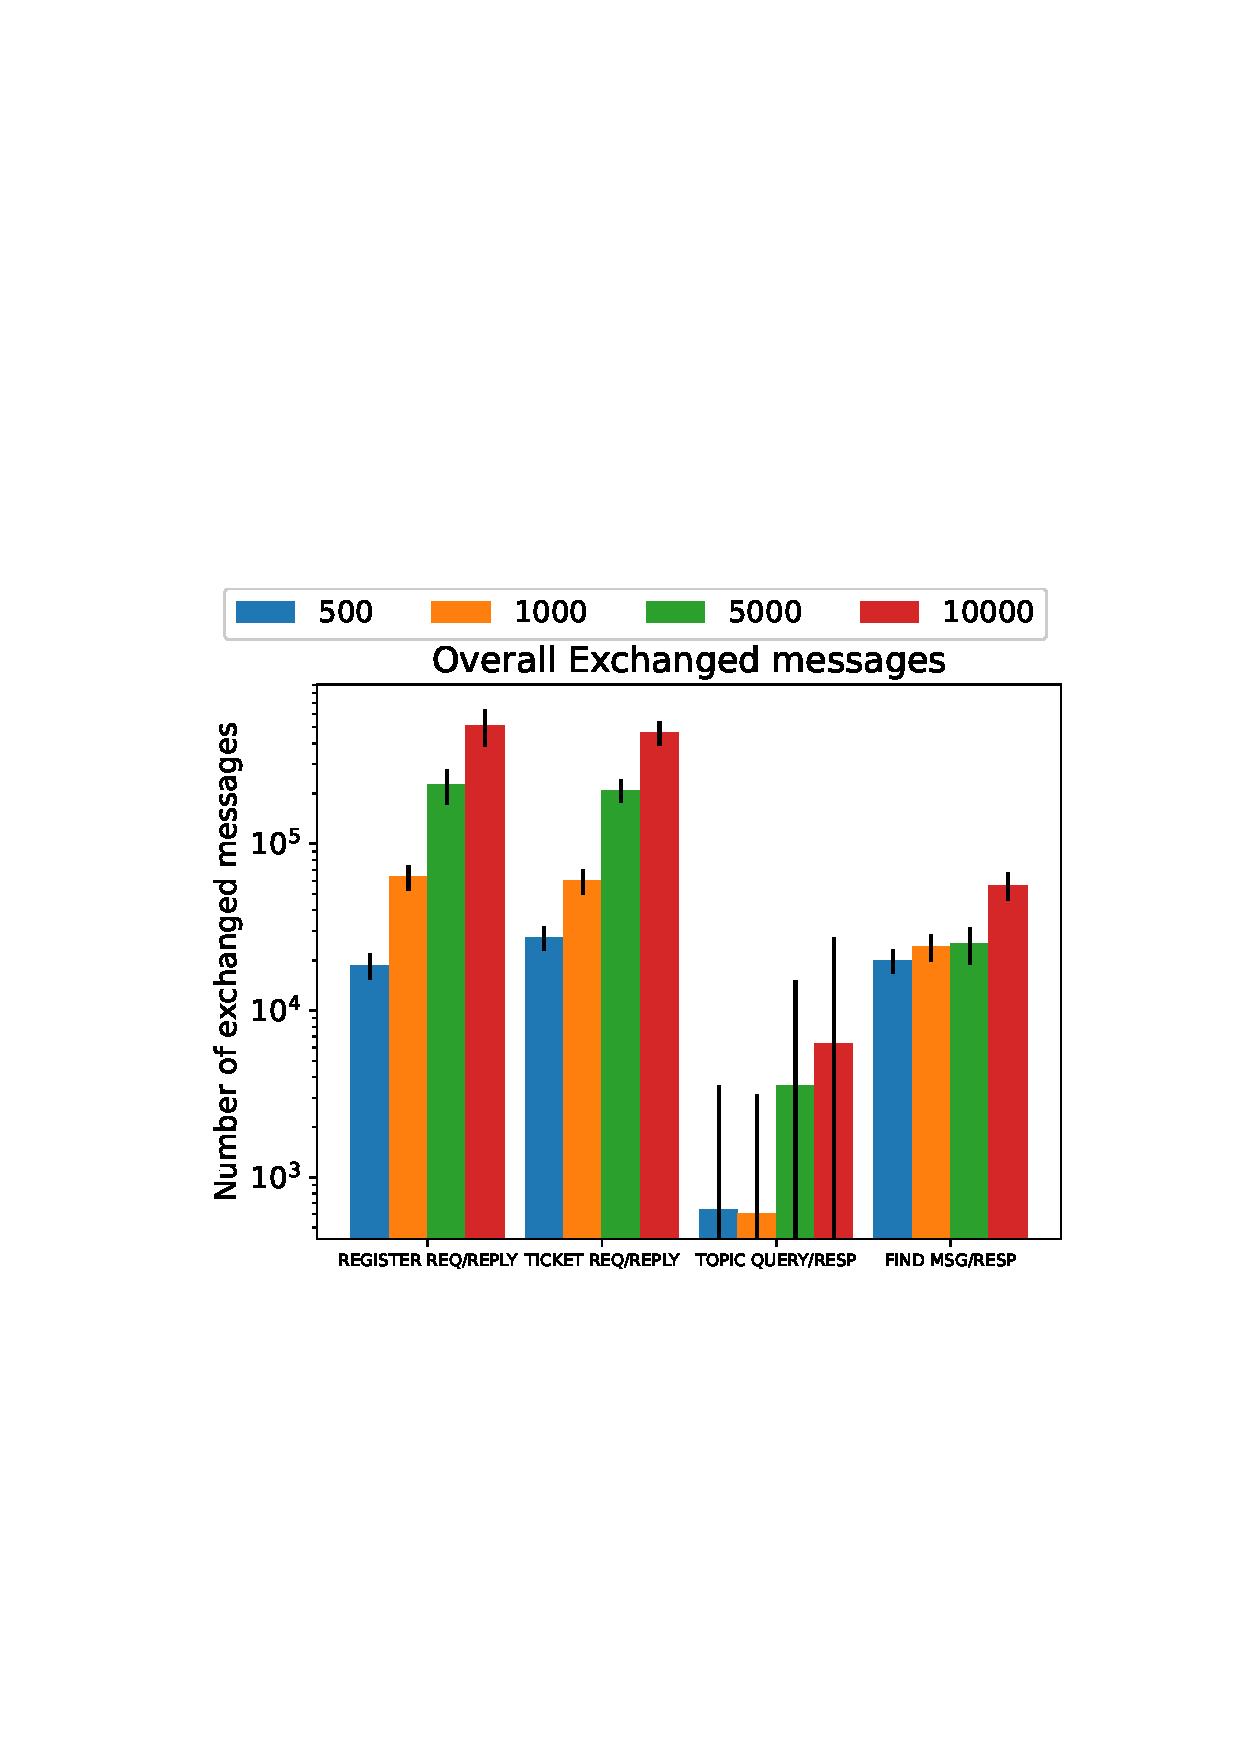
\includegraphics[width=0.23\textwidth]{img/eval/message_quantity.png} 
\label{fig:messages}
} 
\hspace{-0.25cm}
\subfigure[{Message distribution}]{
\includegraphics[width=0.23\textwidth]{img/eval/messages_received2.png} %\hspace{-1.5em}%
\label{fig:msg_distr}
}
 \caption{Traffic load} 
\label{fig:traffic}
\vspace{-0.15in}
\end{figure}   

\paragraph{\bf{Discovery performance}:}

\begin{figure}[!h]
\centering
\subfigure[{Registrant discovery distribution}]{
\includegraphics[width=0.23\textwidth]{img/eval/registrant_distribution.png} 
\label{fig:reg_disc}
} 
\hspace{-0.25cm}
\subfigure[{Time between registration and first discovery}]{
\includegraphics[width=0.23\textwidth]{img/eval/min_time_discovery.png} %\hspace{-1.5em}%
\label{fig:timedisc}
}
 \caption{Discovery} 
\label{fig:discovery}
\vspace{-0.15in}
\end{figure}   

\paragraph{\bf{Table occupancy}:}

\begin{figure}[h!]
\centering
%\epsfig{file=imgs/eval/scen5.pdf, width=0.45\textwidth}
\includegraphics[width=0.3\textwidth]{img/eval/lookup_hopcount.png}
\caption{Lookup hopcount}
\label{fig:hopcount}
\vspace{-0.15in}
\end{figure}


\begin{figure}[h!]
\centering
%\epsfig{file=imgs/eval/scen5.pdf, width=0.45\textwidth}
\includegraphics[width=0.3\textwidth]{img/eval/storage_utilisation.png}
\caption{Storage utilization}
\label{fig:utilisation}
\vspace{-0.15in}
\end{figure}

\paragraph{\bf{Topic Eclipse Attack:}}

- malicious registrations

- eclipsed nodes

- time to register / time to discovery

- hopcount 

\paragraph{\bf{Denial of Service Attack: random topic attack and dos attack}}


- active registrations

- time to register / time to discovery

- hopcount 

\subsection{Testbed evaluation}
"Geth"~\cite{go-ethereum}
